\chapter{Implications on ASEAN policies for better integration and connectivity}

\tab The previous chapters emphasized the benefits of Spatial and Geospatial Technology (SGT) for ASEAN, focusing on a wide range of issues such as logistics, disaster management or public health. This chapter adopts another perspective by looking at the implications on ASEAN policies of the enhancement of ASEAN connectivity through SGT.

\vspace{0.4 cm}

In particular, this chapter will be organized as follows:

\begin{enumerate}

\item What to realize with coordinated ASEAN policies?

\item ASEAN policies for Physical infrastructure

\item ASEAN policy directions for Sustainable value creation from data 

\end{enumerate}


\section{What to realize with coordinated ASEAN policies?}

\tab In order to benefit from the full potential of SGT, ASEAN countries will need to adopt coordinated policies aimed at establishing both a strong infrastructure supporting the use of SGT and a legal framework to organize SGT data utilization, as summarized below.

\begin{enumerate}

\item Physical infrastructure:

\begin{itemize}
\item Space systems: observation, positioning, and communication
\item Ground-based systems: base station networks, satellite communication points, and ground data networks
\end{itemize}

\item Data policies and associated public/industrial policies:

\begin{itemize}
\item Sustainable value creation from data by respecting rights and concerns of data producers and associated stakeholders.
\item Separation of data holdings/ownership and advanced usage by value creators/producers.
\item Sharing benefits among data producers and value creators.
\end{itemize}

\end{enumerate}

The next two sections further develops these necessary political goals.


\section{ASEAN Policies for Physical Infrastructure} \label{infrastructure}

\tab While it has immense potential benefits for the region, the utilization of SGT requires important initial investments for the establishment of highly-advanced  technological infrastructures, both in outer space and at ground level.


\subsection{Space systems: observation, positioning, and communication}

\subsubsection{Earth observation}

\tab Concerning the use of earth observation technologies, we recommend different approaches depending on the kind of application requested.

\begin{enumerate}

\item In the case of \textbf{global earth observation}, the cost of establishing a large constellation of expensive satellites would be unbearable for ASEAN countries, even if united behind this goal. Therefore, it would be beneficial for ASEAN to \textbf{join global earth observation open data clubs} such as the \textit{Group on Earth Observations}.

\item In the case of \textbf{local observation}, ASEAN countries could develop indigenous capabilities through the establishment of regional policies balancing between competition and collaboration. We recommend two approaches, which can be followed in parallel:

	\begin{enumerate}
	\item \textbf{ASEAN satellites}. Joint development/operation of ASEAN satellites by member countries under the banner of ASEAN. We could even imagine the establishment of an ASEAN satellite constellation.
	\item \textbf{National satellites}. Individual development of satellites by member countries, eventually participating in an ASEAN constellation.
	\end{enumerate}

\end{enumerate}

Two supplementary comments can be made regarding the development of local observation capabilities:

\begin{enumerate}

\item A strong focus has been made on the \textbf{importance of the establishment of an ASEAN constellation}. Facing the same challenges on a relatively similar environment and having a solution --- SGT --- transcending by definition national boundaries, it would be highly inefficient for ASEAN member countries to develop in parallel similar technologies without collaborating. Moreover, beyond simple data sharing, the coordinated operation of various ASEAN satellites would improve the efficiency of SGT by allowing an increase in covered area and/or of revisit frequency of the satellites.

\item Beyond regional utilization, the data produced by ASEAN satellites could then be shared in a previously mentioned global earth observation open data club.

\end{enumerate}

\subsubsection{Satellite positioning systems}

\tab

\subsubsection{Satellite communication}

\tab 



\subsection{Ground-based systems}

\tab The second type of infrastructures which will need to be promoted through ASEAN policies are ground systems. In particular, we recommend the development of three different categories of ground systems.

\begin{enumerate}

\item \textbf{Base station networks}. National development of base stations --- necessary for the downlink of data produced by observation satellites or gathered by communication satellites from ground measurement stations --- to form international networks. By having a large network of interconnected base stations, real-time data exchange will be available for ASEAN countries, however conditioned to the interoperability of base stations.

\item \textbf{Satellite communication points}. Individual development with interoperability.

\item \textbf{Ground data networks}. Individual development of ground measurements stations, emitting \textit{in-situ} data towards ASEAN communication satellites. Therefore, the adoption of common data standards will be necessary for the functioning of the full system.

\end{enumerate}

The keyword here in \textbf{interoperability}. Contrary to satellites which are moving in outer space, a neutral area for international law, ground stations will be placed on the exclusive territories of ASEAN member states. Therefore, to use the potential of such a wide network, it is necessary to ensure the \textbf{compatibility} between all infrastructures and facilitate the \textbf{adoption of common standards} throughout ASEAN.


\section{ASEAN policy directions for Sustainable value creation from data} \label{data_util}

\tab This section aims at answering the following question: how to sustain value creation from data, while respecting the rights and concerns of data producers and associated stakeholders?

\vspace{0.4 cm}

To answer this question, we recommend to follow specific policy directions, consisting in the adoption of coordinated data policy for advanced usage. In particular, focus should be placed on:

\begin{enumerate}

\item \textbf{Separating data holdings/ownership and advanced data usage and integration by value creators}, as well as \textbf{respecting rights and concerns of data producers/stakeholders}. In other words, ensuring a smoother flow of data and a clearer responsibility of data usage.

\item \textbf{Sharing the benefits of value creation from data} among data producers and value creators.

\item \textbf{Monitoring and assessing risks and benefits of data usage} and data market competition/concentration in a coherent manner.

\item \textbf{Accelerating human resource development} of value creation.

\end{enumerate}


\begin{figure}[H]
\begin{center}
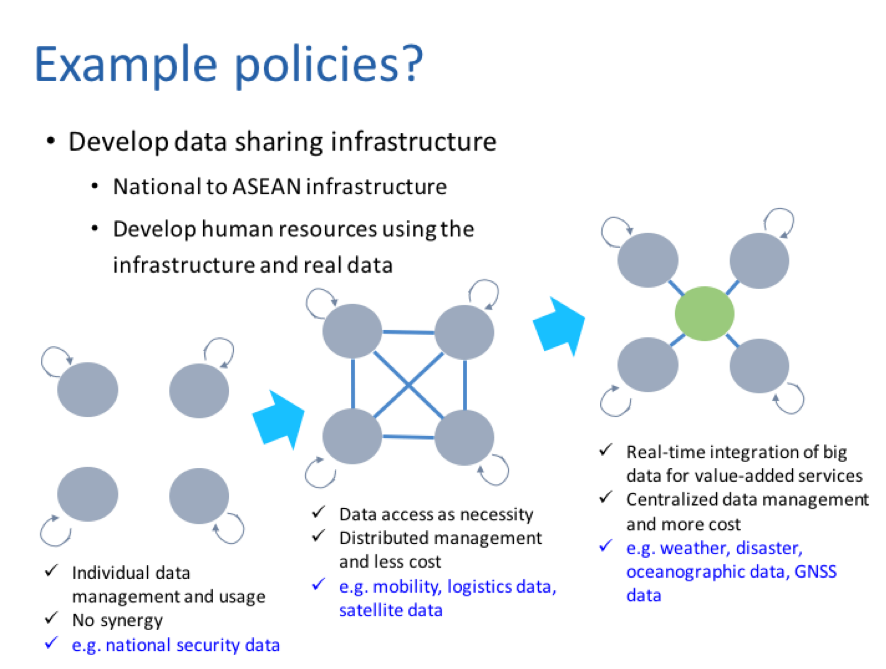
\includegraphics[width = 0.8\linewidth]{Figures/example_policies.png}
\end{center}
\caption{Example policies}
\label{example_policies}
\end{figure}



